\begin{example}
    Consider the following triangle:
    \begin{center}
       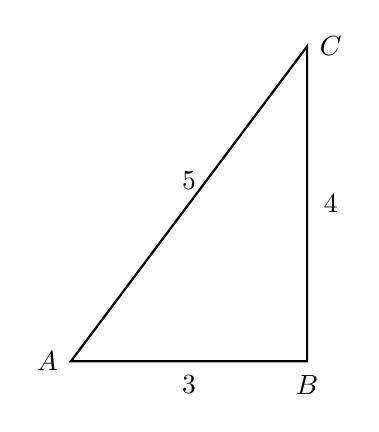
\begin{tikzpicture}
        % Draw the triangle
        \draw[thick] (0, 0) -- (3, 0) -- (3, 4) -- cycle;
        % Label the sides
        \node at (1.5, -0.3) {3};
        \node at (3.3, 2) {4};
        \node at (1.5, 2.3) {5};
        % Label the angles
        \node at (-0.3, 0) {$A$};
        \node at (3, -0.3) {$B$};
        \node at (3.3, 4) {$C$};
    \end{tikzpicture} 
\end{center}
 Clearly, 
$
5 \leq 3 + 4 = 7,
$
indicating the triangle inequality holds true for this example.
\end{example}